\newpage
\section{Kontrastforsterkning}
\label{sec:Kontrastforsterkning}
\subsection{Bakgrunn}
I et bilde er det kontrasten som gjør at vi kan skille et objekt fra bakgrunnen og eventuelle andre objekter.\cite{wiki:kontrast} Et godt eksempel på dette er svart tekst på hvit bakgrunn, hvor kontrasten mellom bokstavene og bakgrunnen er veldig stor. Dette gjør teksten lett å se og lese. I et bilde er det altså fargekontrasten som gjør at vi kan se objekter. Et bilde med høy motivkonstrast\footnote{\url{https://en.wikipedia.org/w/index.php?title=Contrast_(vision)&oldid=941218450}} viser de lyse delene av bildet enda lysere og de mørke delene av bildet enda mørkere. Dette gjør at bildet ser mindre flatt ut for seeren, men gjør i realiteten at det blir mindre detaljer i bildet. Spesielt i de mørkeste og lyseste områdene blir bildene udetaljerte og støyete. Når man skal behandle et bilde vil det være veldig lett å øke kontrastene, mens muligheten for å redusere kontrasten vil være veldig begrenset. 

De fleste metodene for å gjøre en kontrastforsterkning benytter seg av et gråtonehistogram med verdier fra 0 til 255. Dette gråtonehistogrammet beskriver ikke hvor de ulike verdiene finnes på bildet, men beskriver heller fordelingen av grånivåene. Et slikt diagram opprettes ved å telle antall ganger hver en grånivåverdi i bildet oppstår. Deretter deler man med det totale antall piksler i bildet slik at man får en prosentvis andel av hver grånivåverdi. En måte å omdanne et lavkontrastbilde til et høykontrastbilde er ved å gjøre en dynamic range adjustment(DRA)\cite{Contrast:Human}. Dette gjøres ved å strekke grånivåverdiene i bildet slik at histogrammet dekker alle grånivåene mellom 0 og 255, som vist i figur (\ref{Figur 2}).

\begin{figure}[H]
\begin{center}
    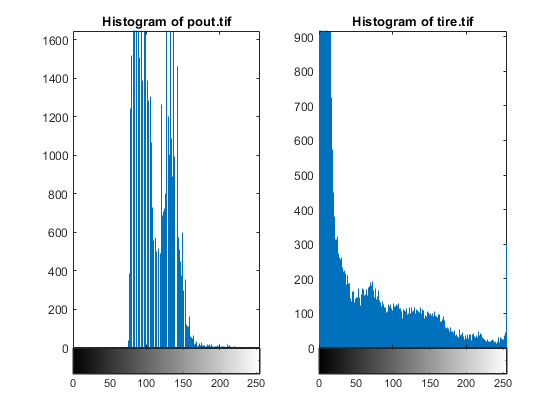
\includegraphics[width=0.7\columnwidth]{bilder/Kontrastforsterkning/graylevelhistogram.png}
    \caption{Graylevel Histogram \label{Figur 2}} \source{MathWorks~\cite{Contrast:histogram}}
\end{center}
\end{figure}
\newpage
\subsection{Implementasjon}
For å finne en mer kontrastert versjon av originalbildet $u_0$ finner vi et bilde som har samme gradient som originalbildet, men forsterket med en konstant $k>1$. Dette gjør vi ved å ta utgangspunkt i likning~(\ref{eq:diffusjon}), og setter $h = k \nabla^2 u_0$. Vi har nå denne likningen
\begin{equation}
\frac{\partial u}{\partial t} = \nabla^2 u - k \nabla^2 u_0.
\label{eq:contrast}
\end{equation}
som løses for $u$. Først finner vi et eksplisitt skjema for hver av de tre fargekanalene i  $u_0$, før vi for hver fargekanal itererer oss frem til en løsning for $u$.

\begin{lstlisting}[language=Python]
u[1:-1, 1:-1, 0] += (0.25 * (u[:-2, 1:-1, 0] + u[2:, 1:-1, 0] + 
                    u[1:-1, :-2, 0] + u[1:-1, 2:, 0] - 
                    4 * u[1:-1, 1:-1, 0]) - k * u0[:,:, 0])
                    
u[1:-1, 1:-1, 1] += (0.25 * (u[:-2, 1:-1, 1] + u[2:, 1:-1, 1] + 
                    u[1:-1, :-2, 1] + u[1:-1, 2:, 1] - 
                    4 * u[1:-1, 1:-1, 1]) - k * u0[:,:, 1])
                    
u[1:-1, 1:-1, 2] += (0.25 * (u[:-2, 1:-1, 2] + u[2:, 1:-1, 2] + 
                    u[1:-1, :-2, 2] + u[1:-1, 2:, 2] - 
                    4 * u[1:-1, 1:-1, 2]) - k * u0[:,:, 2])
\end{lstlisting}
For randbetingelser har vi valgt Neumann, $\frac{\partial u}{\partial n}=\frac{\partial u_0}{\partial n}$. Når en multipliserer $u_0$ med $k$ vil flere pikselverdier $u > 1$ eller $u < 0$, som er utenfor fargeområdet. Derfor må vi klippe verdiene til et lovlig intervall. Dette gjøres før $u$ returneres av funksjonen.
\begin{lstlisting}[language=Python]
u[u < 0] = 0  
u[u > 1] = 1
\end{lstlisting}
Resultatet av vår implementasjon vises i figur \ref{fig:contrast1}, her med \texttt{k=1.7}. Til venstre vises originalbildet slik det blir lastet inn ved hjelp av \texttt{imageio.imread}\footnote{\url{https://pypi.org/project/imageio/}}. Til høyre vises bildet som er kontrastforsterket.
\begin{figure}[H]
\begin{center}
    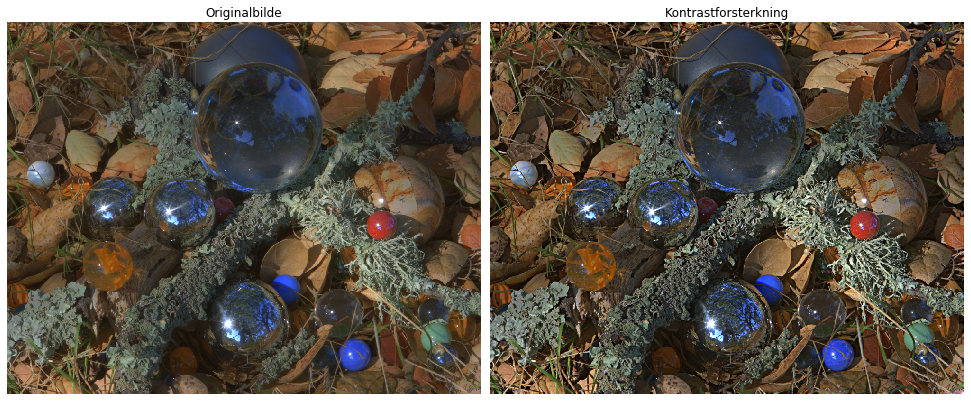
\includegraphics[width=0.72\columnwidth]{bilder/Kontrastforsterkning/kontrast1.png}
     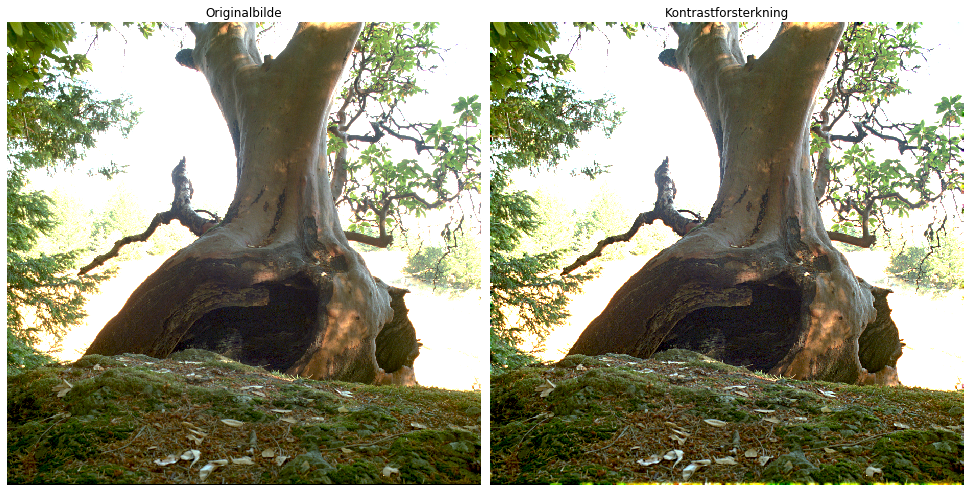
\includegraphics[width=0.72\columnwidth]{bilder/Kontrastforsterkning/kontrast2.png}
    \caption{Kontrastforsterkning \label{fig:contrast1}}
\end{center}
\end{figure}